\documentclass{article}

\usepackage{color,graphicx} 

\begin{document}
\title{GPU --- Architecture \& Programming \\ Assignment 1}
\author{Anirudhan Rajagopalan --- ajr619@nyu.edu}
\maketitle

\newpage

\section{Q3. Bar chart}
The below chart shows the performance of GPU and CPU versions.
\begin{figure}[ht!]
  \centering
  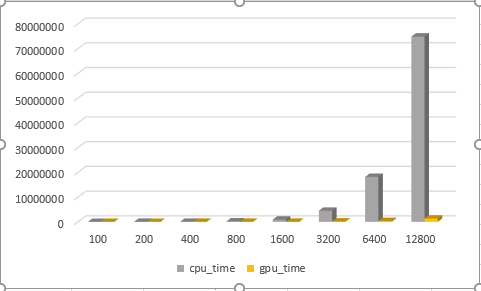
\includegraphics[width=1\textwidth]{capture}
  \caption{GPU and CPU performance.\label{fig:observation}}
\end{figure}


\section{Q4. Observations}
The image~\ref{fig:observation} shows the performance of the GPU and CPU functions.

\begin{figure}[ht!]
  \centering
  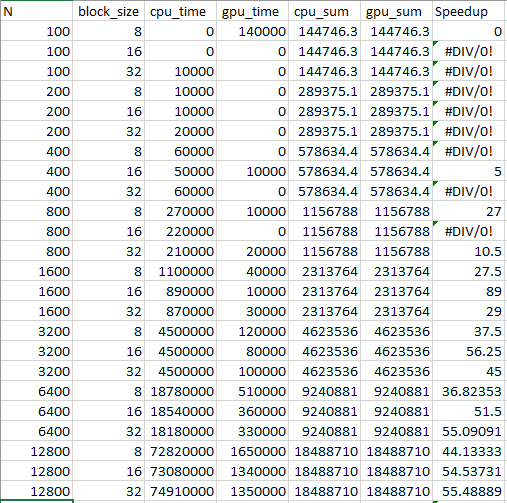
\includegraphics[width=1\textwidth]{speedup}
  \caption{Figure showing performance of GPU and CPU functions for various values of N and various block width.\label{fig:observation}}
\end{figure}

\subsection{When GPU usage is more beneficial}
GPU usage is generally beneficial when the size of our playground is bigger.  For smaller size playground (from 32 to 200), the performance of CPU is better than that of GPU\@.  This is mainly because we need to transfer data across GPU and CPU for doing our calculations and also the GPU overhead.
\subsection{Lowest Speedup}
The lowest speedup (almost in -ve) is observed for N = 100 and block size 32.  As explained above, because of the overhead of copying the data (which is the slowest operation in many GPUs) we have poor performance.
\subsection{Highest Speedup}
The hightest speedup is observed for N = 12800 and block size of 32.  This gives the highest performance as we are using max no\. of threads per block (1024) and also we are making full utilization of the parallel GPUs.

\section{Q5. Effect of number of iterations}
As explained in the section above, we ran a lot of experiments similar to searching a grid of three dimensions.  One dimension for N, the other for block size and the third dimension for iterations.
\begin{enumerate}
\item N = 100, 200, 400, 800, 1600, 3200, 6400, 12800
\item BLOCK\_WIDTH = 8$\times$8, 16$\times$16, 32$\times$32
\item Iterations = 20, 40, 50, 75, 100, 150, 300
\end{enumerate}

We took our best performing (GPU performing) values of N (12800) and block size (32) based on the speedup ratio for all these experiments and tried to run experiments by varying the number of iterations.  The values we got are summarized in Figure~\ref{fig:iterations}

\begin{figure}[ht!]
  \centering
  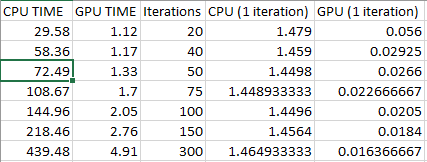
\includegraphics[width=1\textwidth]{iterations}
  \caption{Effect of iterations on cpu and gpu performance.  N = 12800 and block size = 32$\times$32.\label{fig:iterations}}
\end{figure}

As you can see, the utilization of GPU goes up as we add more number of iterations to GPU\@.  This is because GPU will be able to schedule the warps more efficiently as there are more operations to be done.  Thus the execution effeciency goes up.
\end{document}
